% !TEX encoding = UTF-8
% !TEX TS-program = pdflatex
% !TEX root = ../tesi.tex

%**************************************************************
\chapter{Strumenti e tecnologie}
\label{cap:strumenti-e-tecnologie}
%**************************************************************

\intro{Analisi e descrizione delle tecnologie utilizzate}\\

%**************************************************************
\section{Strumenti utilizzati}

\subsection{Ambiente di sviluppo}
Durante le 8 settimane di stage, mi è stata assegnata una macchina con sistema operativo Windows 10 64 bit per svolgere il tirocinio universitario. Mi è stato richiesto di utilizzare Virtual Box per poter creare l'ambiente di sviluppo con sistema operativo Debian 10.10 (Buster). \newline{} Virtual Box è un software gratuito e open source per l'esecuzione di macchine virtuali per architettura x86 e 64bit che supporta Windows, GNU/Linux e macOS come sistemi operativi host, ed è in grado di eseguire Windows, GNU/Linux, OS/2 Warp, BSD come ad esempio OpenBSD, FreeBSD e infine Solaris e OpenSolaris come sistemi operativi guest.\newline{}
Nella macchina virtuale in seguito mi è stato consigliato di utilizzare PyCharm come strumento per lo sviluppo del prodotto.\newline{}
PyCharm è un IDE integrato multi-piattaforma per Python; è un software distribuito sotto i termini della Apache License nella sua versione "Community".
\begin{figure}[!h]
    \begin{minipage}{.5\textwidth} 
        \centering 
        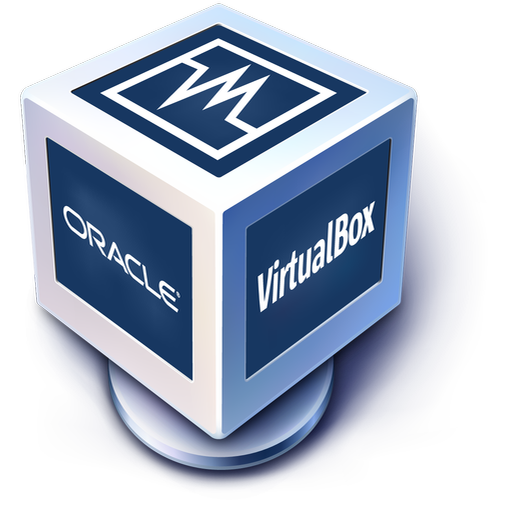
\includegraphics[width=.4\linewidth]{logo-virtualbox.png} 
        \caption{Logo Virtualbox} 
        \label{fig:virtualbox} 
    \end{minipage}% 
    \begin{minipage}{.5\textwidth} 
        \centering 
        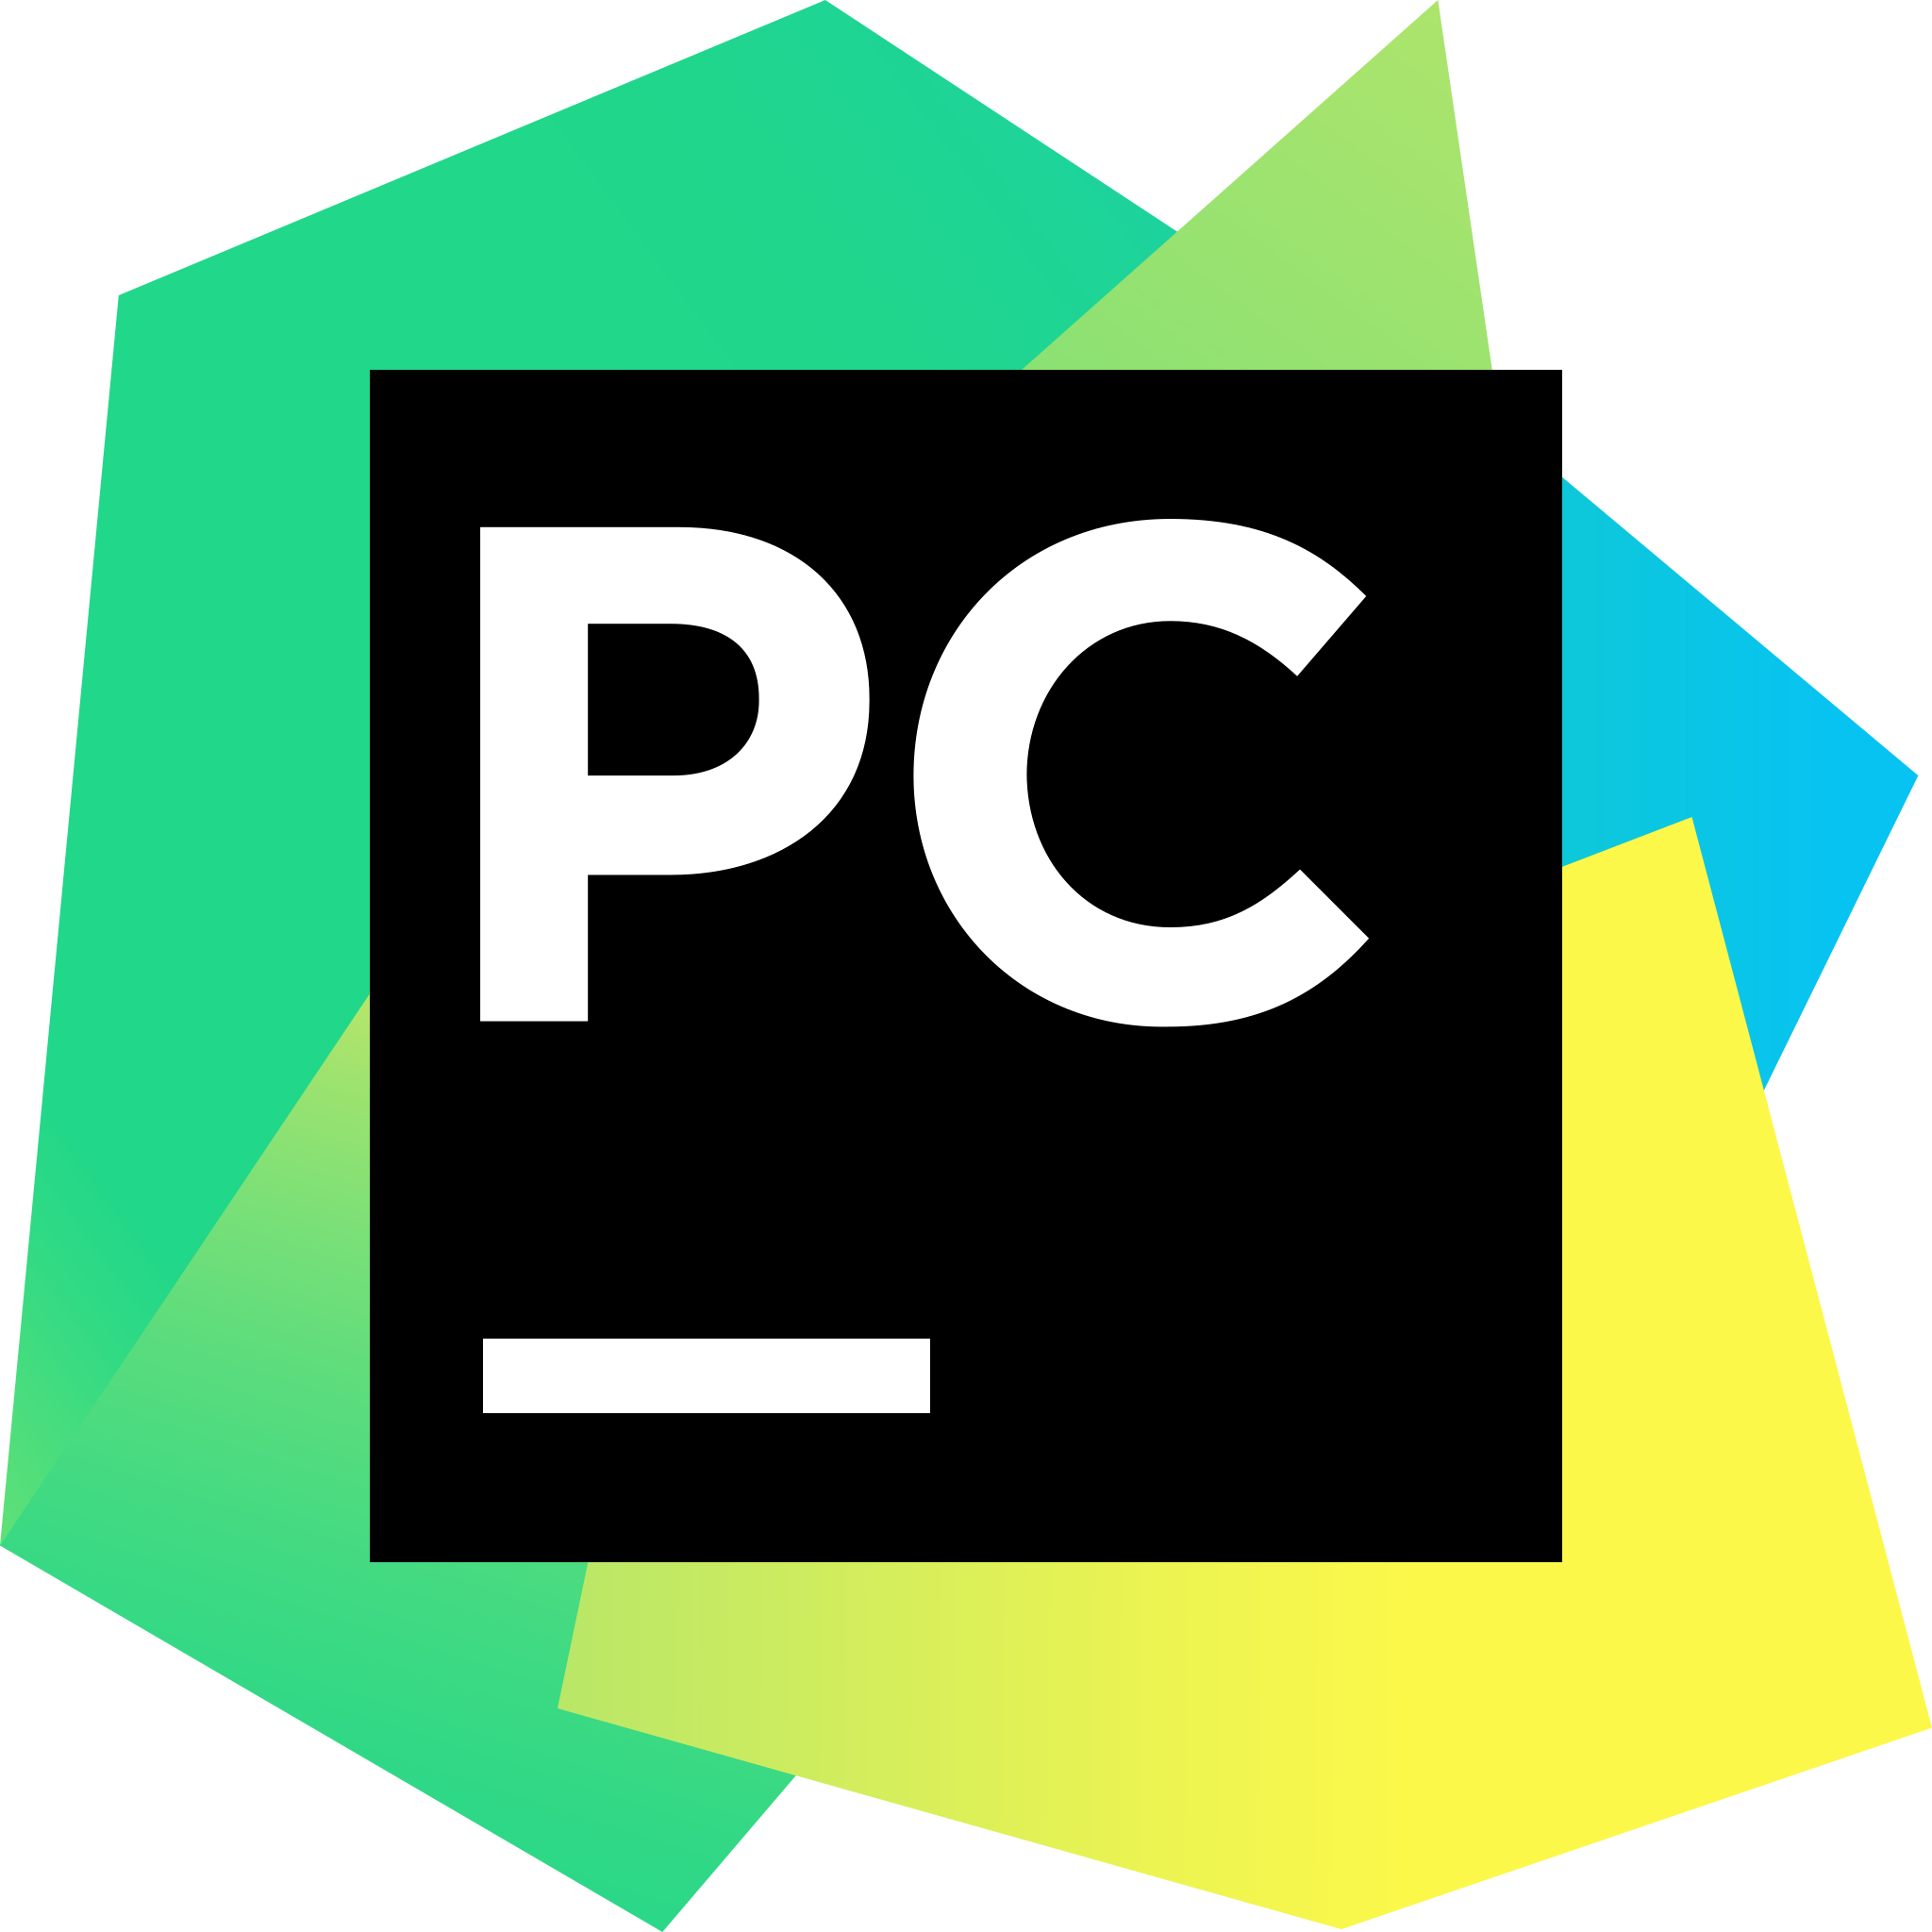
\includegraphics[width=.4\linewidth]{logo-pycharm.png} 
        \caption{Logo PyCharm} 
        \label{fig:pycharm} 
    \end{minipage}  
\end{figure}

\subsection{Strumenti di versionamento}

L’azienda, per tutti i suoi prodotti, adotta strumenti per il controllo di versione, nello specifico Git. Git è un software di controllo versione distribuito utilizzabile da interfaccia a riga di comando, creato da Linus Torvalds nel 2005. È stato scelto rispetto ad altri strumenti di Version Control System (VCS) perché favorisce lo sviluppo non lineare, per il supporto di branching e merging e perché comprende strumenti specifici per visualizzare e navigare una cronologia di sviluppo non lineare. Infine, come servizio di hosting web-based, è stato utilizzato GitLab.

\begin{figure}[!h]
    \begin{minipage}{.5\textwidth} 
        \centering 
        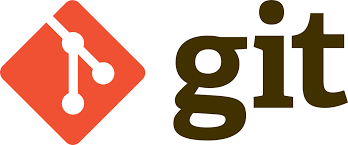
\includegraphics[width=.4\linewidth]{logo-git.png} 
        \caption{Logo Git} 
        \label{fig:git} 
    \end{minipage}% 
    \begin{minipage}{.5\textwidth} 
        \centering 
        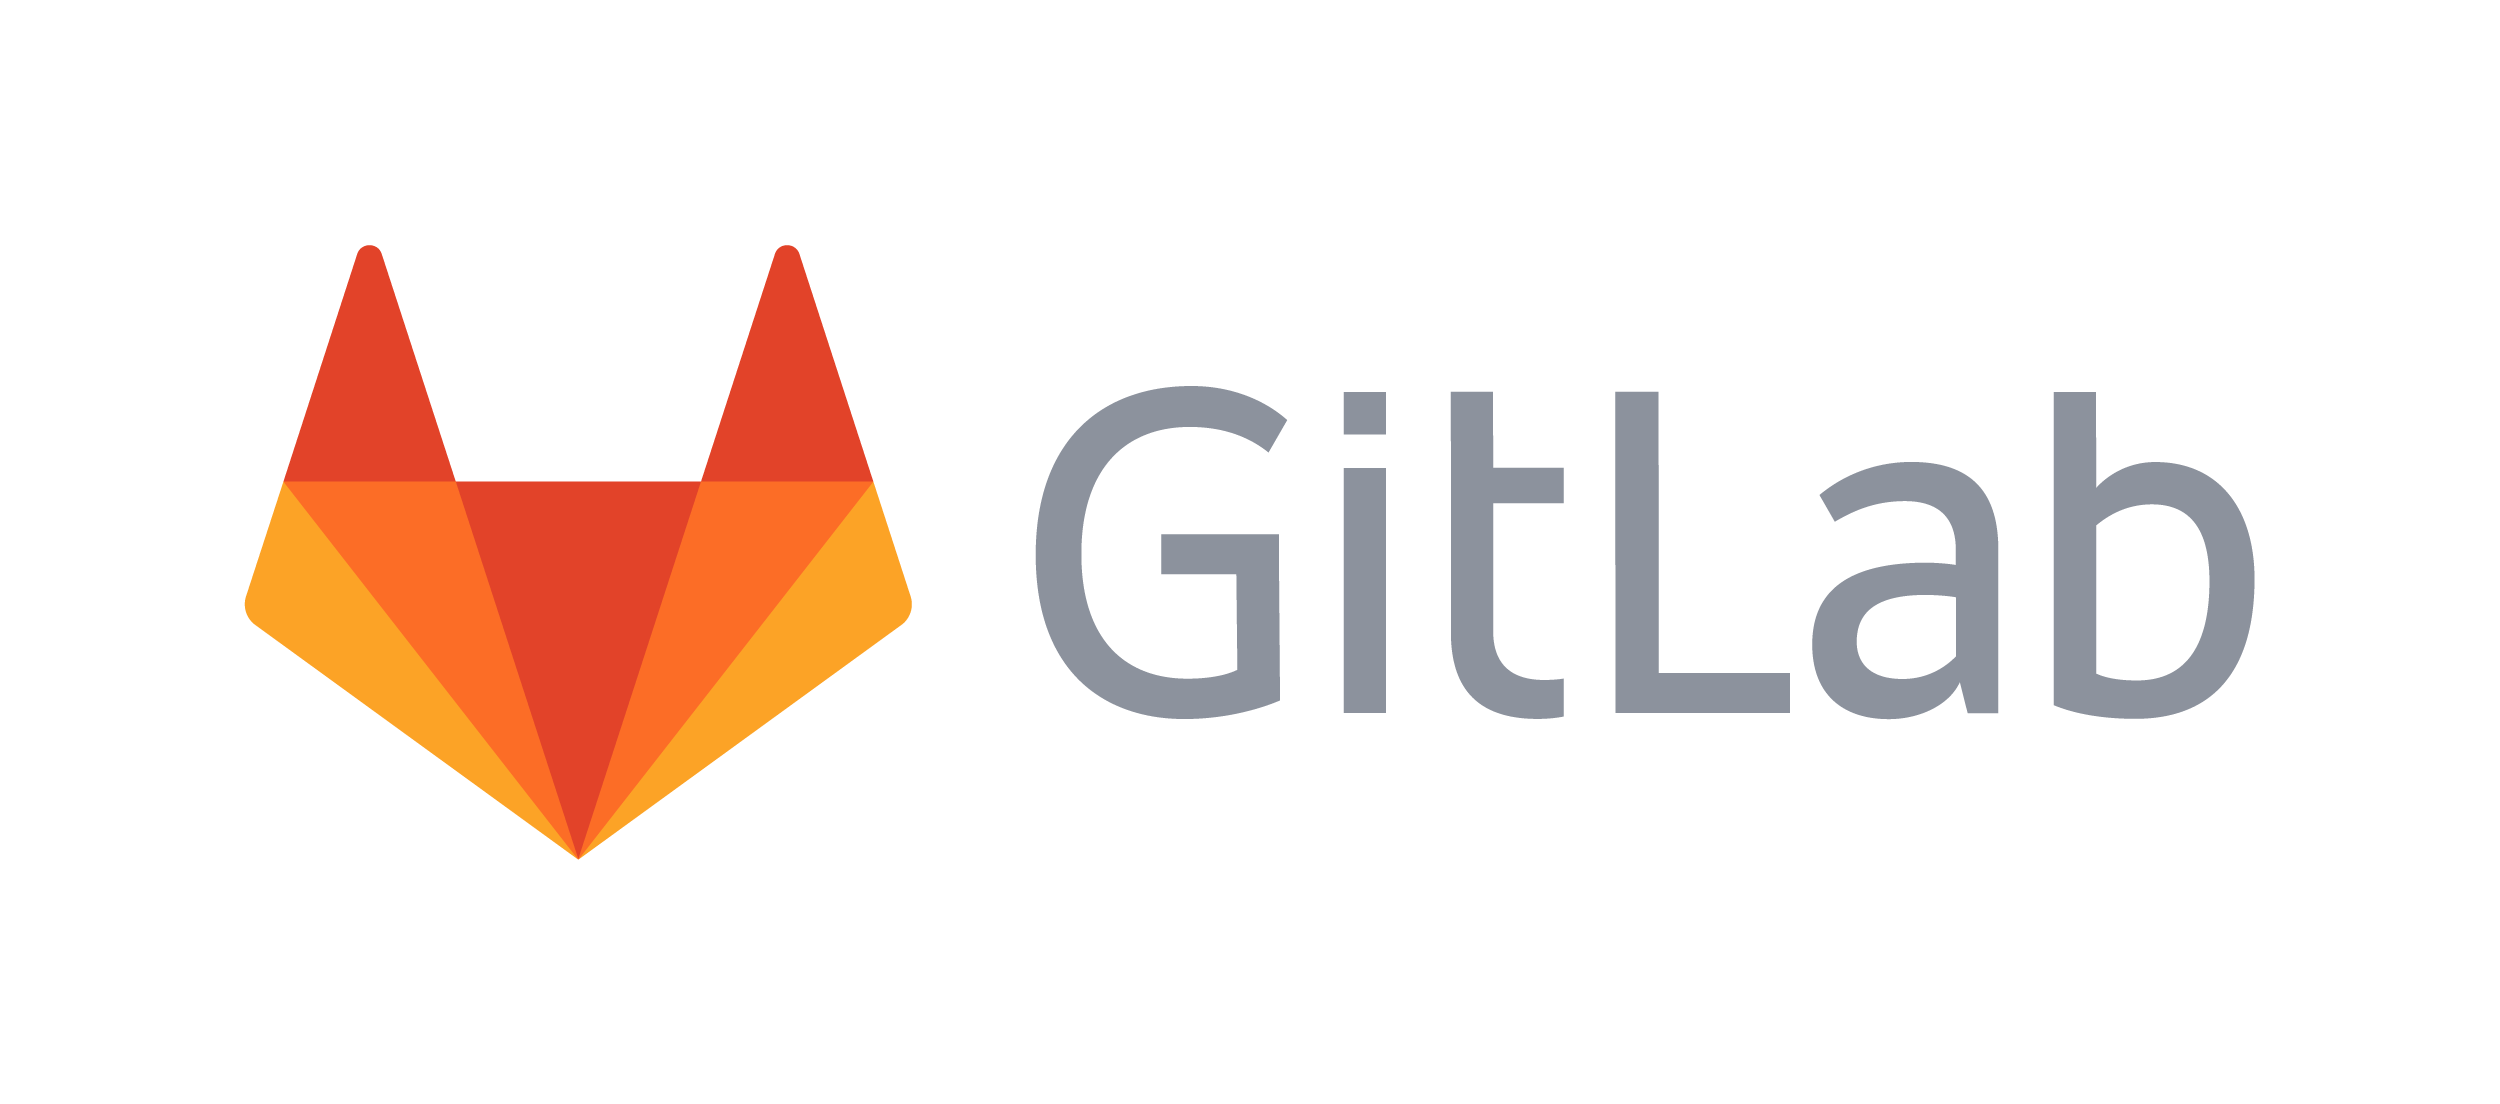
\includegraphics[width=.4\linewidth]{logo-gitlab.png} 
        \caption{Logo GitLab} 
        \label{fig:gitlab} 
    \end{minipage}  
\end{figure}

\subsection{Strumenti aziendali}

Per quanto riguarda la comunicazione con il tutor aziendale, è stato utilizzati Microsoft Teams e Whatsapp. Entrambi gli strumenti sono stati utililzzati per comunicare con il tutor e il personale aziendale durante tutto il tirocinio universitario.

\begin{figure}[!h]
    \begin{minipage}{.5\textwidth} 
        \centering 
        
\includegraphics[width=.4\linewidth]{logo-teams.png} 
        \caption{Logo Microsoft Teams} 
        \label{fig:teams} 
    \end{minipage}% 
    \begin{minipage}{.5\textwidth} 
        \centering 
        
\includegraphics[width=.4\linewidth]{logo-whatsapp.png} 
        \caption{Logo WhatsApp} 
        \label{fig:whatsapp} 
    \end{minipage}  
\end{figure}

\subsection{Altri strumenti}

%**************************************************************
\section{Tecnologie utilizzate}

\subsection{Linguaggi}

\subsection{Framework}
Selenium e robe per test 

%**************************************************************